\documentclass[parskip=full]{scrartcl}

\usepackage[utf8]{inputenc}			% Umlaute, Sonderzeichen
\usepackage[ngerman]{babel}			% deutsche Sprache
\usepackage{enumitem}				% Listen
\usepackage{graphicx}				% Grafiken
\usepackage{hyperref}				% Hyperlinks
\usepackage[nonumberlist]{glossaries}		% Glossar
\usepackage{amsmath}
\usepackage{pdfpages}				% PDF einbinden

% Hurenkinder und Schusterjungen verhindern
\clubpenalty10000
\widowpenalty10000
\displaywidowpenalty=10000

\DeclareRobustCommand{\glossfirstformat}[1]{\textit{#1}}	% der erste Verweis im Dokument auf ...
\renewcommand*{\glsdisplayfirst}[4]{\glossfirstformat{#1#4}}	% ... einen Glossarbegriff wird kursiv markiert

% Kriterien sollen nicht kursiv erscheinen
\makeatletter
\renewcommand{\@begintheorem}[2]{\trivlist
	\item[\hskip \labelsep{\bfseries #1\ #2}]}
\makeatother


\makenoidxglossaries

\newglossaryentry{RasPi}{
	name=Raspberry Pi,
	plural=Raspberry Pis,
	description={Der Raspberry Pi ist ein Einplatinencomputer. In diesem Projekt dient der Raspberry Pi als Hardwareplattform, um Messwerte aus angeschlossenen Sensoren auszulesen}
}

\newglossaryentry{PhyPiDAQ}{
	name=PhyPiDAQ,
	description={PhyPiDAQ ist ein Framework zur Erfassung und Analyse von Messwerten mit einem Raspberry Pi. Siehe auch Abschnitt 4.3 ,,PhyPiDAQ`` sowie \url{https://github.com/GuenterQuast/PhyPiDAQ}}
}

\newglossaryentry{Science Labs}{
	name=Science Labs,
	description={Ein Science Lab ist ein Arbeitsplatz, welcher Schülern ermöglicht, wissenschaftliche Forschungen unter kontrollierten Bedingungen durchzuführen} 
}

\newglossaryentry{opensource}{
	name=Open Source,
	description={Software, deren Quelltext öffentlich eingesehen eingesehen werden kann, wird als ,,Open Source`` bzw. ,,quelloffen`` bezeichnet} 
}

\newglossaryentry{osl2}{
	name=OSL\textsuperscript{2},
	description={Open-Source-Lehrsoftware-Labor, siehe \url{https://formal.iti.kit.edu/projects/oslsl/?lang=de}}
}

\newglossaryentry{dragdrop}{
	name=Drag and Drop,
	description={Methode, um mit grafischen Benutzeroberflächen zu interagieren. Dabei wird ein Objekt erst mit der Maus festgehalten und an einen anderen Ort gezogen. Durch das Lösen der Maustaste wird das Objekt platziert}
}

\newglossaryentry{click}{
	name=Click,
	description={Betätigen der linken Maustaste}
}

\newglossaryentry{transformation}{
	name=Transformation,
	plural={Transformationen},
	description={Bausteine vom Typ Transformation haben einen oder mehrere Eingänge sowie einen oder mehrere Ausgänge. Für jeden Ausgang kann  ein Transformationsbaustein eine Vorschrift zur Berechnung eines Ausgangswertes aus einem Satz von Eingangswerten beinhalten. Eine Berechnungsvorschrift soll durch eine mathematische bzw. logische Funktionen oder durch eine programmtechnisch definierte Verarbeitung definiert werden können}
}

\newglossaryentry{konfigdata}{
	name=Konfigurationsdatei,
	plural=Konfigurationsdateien,
	description={Können das Messverhalten anpassen, beispielsweise die Anzahl der Messungen pro Zeiteinheit. Für jeden Sensor gibt es eine eigene Konfigurationsdatei}
}

\newglossaryentry{sensor}{
	name=Sensor,
	plural={Sensoren},
	description={Der Begriff ,,Sensor`` bezeichnet ein technisches Bauteil, welches physikalische Größen misst und analoge oder digitale Messwerte liefert. In unserer Anwendung werden Sensoren abstrakt als grafische Bausteine eines Messkonfiguration präsentiert. Ein solcher (logischer) Sensorbaustein muss alle Informationen referenzieren können, die zum Ansprechen eines tatsächlichen Sensors benötigt werden. Da ein Messgerät Ausgänge bzw. Messkanäle haben kann, muss ein Sensorbaustein mindestens einen oder auch mehrere Ausgänge haben. Eingänge besitzt ein Sensorbaustein nicht}
}

\newglossaryentry{messdaten}{
	name=Messdaten,
	description={Daten, welche die Anwendung von einem Sensor (über PhyPiDAQ-Schnittstelle) oder direkt aus einer Datei erhält}
}

\newglossaryentry{darstellung}{
	name=Darstellung,
	plural={Darstellungen},
	description={Bausteine vom Typ Darstellung haben einen oder mehrere Eingänge. Ein Darstellungsbaustein soll definieren können, wie ein Satz von Eingangswerten die Erstellung bzw. Aktualisierung einer Darstellung beeinflusst. Ausgänge besitzt ein Darstellungsbaustein nicht}
}

\newglossaryentry{python3}{
	name=Python 3,
	description={Python ist eine Skriptsprache, die auf dem Raspberry Pi als Standardsprache zur Programmierung vorgesehen ist. Python wurde zur Implementierung von PhyPiDAQ verwendet}
}

\newglossaryentry{JVM}{
	name={Java Virtual Machine},
	description={Die Java Virtual Machine (JVM) ist eine Plattform für die Ausführung von Java-Software, die von der Firma Oracle für alle gängigen Betriebssysteme bereitgestellt wird}
}

\newglossaryentry{DSGVO}{
	name=DSGVO,
	first={Datenschutz-Grundverordnung (DSGVO)},
	description ={Datenschutz-Grundverordnung der Europäischen Union vom 25. Mai 2018}
}

\newglossaryentry{Musskriterien}{
	name=Musskriterien,
	description ={Werden zusammen mit Soll- und Wunschkriterien bei der Abnahme eines Softwareprodukts überprüft und haben während der Entwicklung höchste Priorität. 
	Dass ein Musskriterium in den nachfolgenden Projektphasen nicht umgesetzt wird, ist nur dann zulässig, falls unerwartet unausweichliche Probleme bei der Umsetzung auftreten. 
	In diesem Fall ist es erforderlich, dass diese Probleme sehr genau dokumentiert werden}
}

\newglossaryentry{Sollkriterien}{
	name=Sollkriterien,
	description ={Werden zusammen mit Muss- und Wunschkriterien bei der Abnahme eines Softwareprodukts überprüft und haben während der Entwicklung mittlere Priorität. 
	Falls ein Sollkriterium umgesetzt werden kann, dann muss es nach Möglichkeit auch realisiert werden. 
	Falls ein Sollkriterium in den nachfolgenden Projektphasen nicht umgesetzt werden kann, so muss dies dokumentiert und begründet werden}
}

\newglossaryentry{Wunschkriterien}{
	name=Wunschkriterien,
	description ={Werden zusammen mit Muss- und Sollkriterien bei der Abnahme eines Softwareprodukts überprüft und haben während der Entwicklung eine niedrige Priorität. 
	Je nach Resourcenlage können sie nach Bearbeitung aller Muss- und Kannkriterien umgesetzt werden. 
	Falls ein Wunschkriterium nicht umgesetzt wird, so muss dies nicht begründet werden}
}

\newglossaryentry{Abgrenzungskriterien}{
	name=Abgrenzungskriterien,
	description ={Abgrenzungskriterien beschreiben Aspekte, die explizit nicht umgesetzt werden sollen.}
}

\newglossaryentry{BenOber}{
	name=Benutzeroberfläche,
	description = {Steht für die Oberfläche, die der Benutzer verwendet um die Anwendung zu bedienen}
}

\newglossaryentry{UI}{
	name=UI,
	description={engl. User Interface; siehe: Benutzeroberfläche}
}

\newglossaryentry{GrafBenOber}{
	name=grafische Benutzeroberfläche,
	description = {Eine Benutzungsschnittstelle, die eine Anwendung durch Fenster, grafische Symbole, Menüs und Mauszeiger bedienbar macht}
}

\newglossaryentry{GUI}{
	name=GUI,
	description={engl. Graphical User Interface; siehe: Grafische Benutzeroberfläche},
}

\newglossaryentry{Konfigurationsbaustein}{
	name=Konfigurationsbaustein,
	plural=Konfigurationsbausteine,
	description ={Teil einer Messkonfiguration, der eine Teilaufgabe bestimmten Typs erfüllen kann. Es gibt Sensorbausteine, Konfigurationsbausteine und Darstellungsbausteine. Liegt am Ausgang eines Bausteins ein Wert an, so kann dieser an den Eingang eines nachgelagerten Bausteins weitergeleitet werden}
}

\newglossaryentry{Benutzerkonfiguration}{
	name =Messkonfiguration,
	plural=Messkonfigurationen,
	description ={Gerichteter zyklenfreier Graph mit Knoten vom Typ Sensor, Transformation oder Darstellung. Hierbei ist zu beachten, dass Sensoren keine Eingangskanten und Darstellungen keine Ausgangskanten haben dürfen}
}

\newglossaryentry{Bausteinprototyp}{
	name=Bausteinprototyp,
	plural=Bausteinprototypen,
	description={Baustein, von dem eine Kopie angelegt wird, wenn der Benutzer ein neues Baustein-Exemplar einem Entwurf hinzufügen möchte}
}

\newglossaryentry{Messlauf}{
	name=Messlauf,
	plural=Messläufe,
	description={Zeitabschnitt, in dem zu definierten Zeitpunkten an allen Bausteinen eines Entwurfs sukzessive die Werte an allen Ausgängen und Eingängen bestimmt werden}
}

\newglossaryentry{Stand-Alone-Kommunikation}{
	name={Stand-Alone-Kommunikation},
	description={Bezeichnet im Kontext unseres Software-Projekt die systeminterne Kommunikation innerhalb eines Betriebssystems, beispielsweise per Inter-Prozess-Kommunikation (IPC)}
	}


\newglossaryentry{Local-Loop}{
	name={Local-Loop},
	description={Bezeichnet einen virtuellen Netzwerkadapter, der Pakete, die durch ihn verschickt werden, unmittelbar danach auch wieder empfängt.}
}

\newglossaryentry{Model-View-Controller}{
	name={Model-View-Controller},
	description={Architekturmuster, dass die Software in die drei Komponenten: Model, View und Controller unterteilt. Dadurch sollen die einzelnen Komponenten unabhängig von einander verändert werden können.}
}

\newglossaryentry{JHotDraw}{
	name={JHotDraw},
	description={JHotDraw ist ein Open-Source, Java-basiertes Framework zur Erstellung von grafischen Editoren. Durch die einfachere Unterstützung von Drag-and-Dop, als komplexere Frameworks eine gute Alternative.}
}

\newglossaryentry{allgemeinen Bausteinprototyp-Informationen}{
	name = {allgemeinen Bausteinprototyp-Informationen},
	description = {Dazu gehören folgende Eigenschaften: Name, Typ, Configurations ID, Initialisierungs ID, Nutzerinformationen (Hilfetext)}
}

\newglossaryentry{SWT}{
	name = {Standard Widget Toolkit},
	description = {Ein GUI Framework.}
}

\newglossaryentry{GEF}{
	name = {Graphical Editing Framework},
	description = {Ein GUI Framework.}
}

\newglossaryentry{Swing}{
	name = {Swing},
	description = {Ein GUI Toolkit.}
}

\newglossaryentry{AWT}{
	name = {Abstract Window Toolkit},
	description = {Ein GUI Toolkit.}
}

\newglossaryentry{Presenter}{
    name = {Presenter},
    description = {Presenter bezieht sich auf die gleichnahmige Komponente in einem Model-View-Presenter.}
}
\subject{Implementierungsdokumentation}
\title{Definition und Durchführung~von Messwertverarbeitung für~den~Physikunterricht auf~Basis~eines~Raspberry~Pis}
\subtitle{Version 1.0.0}
\author{David Gawron \and Stefan Geretschläger \and Leon Huck \and Jan Küblbeck \and Linus Ruhnke}
\date{\today}


\begin{document}

\maketitle

\clearpage
\tableofcontents 					% generate pdf twice to update

\clearpage
\section{Ziel der Implementierungsdokumentation} \label{einleitung}

Im sogenannten Wasserfallmodell folgte nach der Anforderungsanalyse und dem Entwurf nun die Implementierung der Softwarewaremodule als dritte Entwicklungsphase. Dieses Dokument soll den Entwicklungsstand am Ende dieser Phase sowie den Verlauf der Phase wiedergeben. Hierbei werden das erstellten Pflichtenheft und die zuvor erstellten UML-Diagrammen herangezogen, und der Stand der Entwicklung wird zu den Inhalten dieser Artefakte in Bezug gesetzt.

\clearpage
\section{Ausarbeitungsstand der Abnahmekriterien} \label{Ausarbeitungsstand}

Im Folgenden werden die Muss-, Soll- und Wunschkriterien aus dem Pflichtenheft herangezogen, das in der ersten Phase des Projekts entstanden ist. Es findet eine Bestandsaufnahme statt, inwieweit die Kriterien erfüllt sind. 

Falls das Softwareprodukt ein Musskriterium nicht wie im Pflichtenheft beschrieben aufweist, so führt dieses Dokument detailliert die Ursachen und Gründe hierfür auf. Falls das Softwareprodukt ein Sollkriterium nicht wie im Pflichtenheft beschrieben aufweist, so beschreibt dieses Dokument zwar nicht in jedem Detail, aber hinreichend informativ die Ursachen und Gründe hierfür. Nicht umgesetzte Wunschkriterien werden lediglich benannt, aber nicht hinterfragt. 

\subsection{Entwurf von Messkonfigurationen}
Es fand ein Fallback statt. Die Messkonfigurationen werden nicht wie gewünscht graphisch durch ein Drag- and Drop Feld erstellt, sondern müssen textuell eingegeben werden. Dadurch verändert sich auch die Betrachtung, wie und ob die folgenden Kriterien überhaupt erfüllt werden können.

\begin{description}
\item[MK 1] Das Musskriterium "`Hinzufügen eines Bausteins aus dem Prototypen-Feld zu der Messkonfiguration"' ist nicht erfüllt. Durch den Fallback zu einem textuellen Messkonfigurationsfeld ist ein direktes Platzieren nicht mehr möglich. Der Benutzer kann zwar anhand der Daten des Bausteinprototypen einen solchen im Konfigurationsfeld erstellen, aber ein direktes Platzieren einer Kopie ist nicht möglich. Die Priorität in der zweiten Hälfte der Implementierungsphase lag darin, eine funktionierende Minimalanwendung zu erstellen, so dass überhaupt ein Prototyp zur Veränderung und Speicherung eines Datenstroms erstellt wird. Die Entscheidung auf den Fallback zurück zu greifen, fiel in der zweiten Hälfte der Implementierungsphase. In der ersten Hälfte wurde viel Zeit damit verbracht ein geeignetes Gui-Framework für eine Drag- and Drop Anwendung zu suchen und sich darin einzuarbeiten. Die Einarbeitungszeit war dabei sehr Zeit fordernd, so dass sich das komplette Projekt verzögerte und drohte zu scheitern.
\item[MK 2] Das Musskriterium "`Anpassen von wichtigen funktionalen Bausteineigenschaften"' ist teilweise erfüllt. Der Benutzer kann die Eigenschaften des Bausteins verändern, allerdings ist das Verändern der Position im Konfigurationsfeld nicht wirklich möglich. Der Benutzer kann zwar die Reihenfolge der Bausteine innerhalb der textuellen Konfiguration verändern, allerdings haben die Bausteine im Model keine Positionsattribute und es gibt auch kein Konfigurationsfeld mit Positionskoordinaten. Darum ist dieser Teil des Musskriteriums nicht erfüllt. 
\item[MK 3] Das Musskriterium "`Löschen eines Bausteins aus der Messkonfiguration"' ist erfüllt, da der Benutzer die Textuelle Repräsentation eines Bausteins aus der Messkonfiguration entfernen kann und dieser, nach einem Neuladen, auch so im Model entfernt wird.
\item[MK 4] Das Musskriterium "`Erstellen einer Verbindung"' ist umgesetzt. Der Benutzer kann ein Kanaltupel der Liste an Verbindungen hinzufügen und somit eine Verbindung der Messkonfiguration hinzu fügen. 
\item[MK 5] Das Musskriterium "`Löschen einer Verbindung"' ist erfüllt. Der Benutzer kann eine Verbindung aus der Liste der Verbindungen löschen, in dem er das entsprechende Kanaltupel löscht.
\item[SK 1] Das Sollkriterium "`Undo-Redo-Funktion"' ist nicht umgesetzt. Die Messkonfiguration wird textuell erstellt und der Editor unterstützt keine Undo-Redo-Funktion. 
\item[WK 1] Das Wunschkriterium "`Hinzufügen, Bearbeiten und Löschen von ergänzender Informationen zu der Messkonfiguration durch den Benutzer"' ist nicht umgesetzt.
\end{description}
\subsection{Handhabung von Bausteinprototypen}

\begin{description}
	\item[SK 2] Der Benutzer ist in der Lage die Eigenschaften der Bausteinprototypen einzusehen. Jedoch ist die Ansicht auf das Anzeigen der \gls{allgemeinen Bausteinprototyp-Informationen} beschränkt. Der Grund hierfür ist die Anbindung von dem Model an die GUI. Dadurch ist es aktuell nur möglich mit den allgemeinen Bausteinprototyp-Informationen zu arbeiten. Dementsprechend ist das Anzeigen der speziellen Eigenschaften, der Bausteinprototypen, nicht möglich.
	\item[SK 3] Das Kopieren der Bausteinprototypen ist möglich. Auch das Anpassen der allgemeinen Eigenschaften ist möglich. Jedoch können keine generischen Bausteinprototypen erstellt werden. Dafür wäre die Erstellung einer allgemeinen Vorläge nötig gewesen. Diese Erweiterung hätte dem Nutzer jedoch keine weitere Funktionalität geboten. Aus diesem Grund haben wir uns dazu entschieden die Funktion erst in einer eventuellen Erweiterung der Anwendung zu integrieren.
	\item[WK 2] Die Verwendung von erweiternder Software, über eine Schnittstelle, ist nicht mehr vorgesehen. Externe Software kann weiterhin zur Erstellung von Yaml-Dateien genutzt werden. Die so entstandenen Yaml-Dateien können über die Lade-Funktion der Anwendung aufgerufen und anschließend verwendet werden.
	\item[SK 4] Die Anwendung unterscheidet in ihrer jetzigen Form nicht zwischen Benutzerdefinierten- und System-Bausteinen. Deshalb ist es auch hier nur möglich die allgemeinen Eigenschaften der Bausteinprototypen zu ändern.
	\item[SK 5] Das Löschen von erstellten Bausteinprototypen ist ermöglicht.
\end{description}
		
\subsection{Gewährleisten von Persistenz}

\begin{description}
\item[MK 6] Das Kriterium ist erfüllt. Die verwendeten Bausteine und ihre Anordnung, also die Messkonfiguration, kann in einer Datei gespeichert werden.
\item[MK 7] Das Kriterium ist erfüllt. Messkonfigurationen können aus Dateien geladen werden.
\item[SK 6] Das Kriterium ist nicht erfüllt, da keine neuen Prototypen in der Anwendung erstellt werden können. (Siehe SK 3)
\item[SK 7] Bausteine werden aus Dateien geladen, die jedoch nur außerhalb der Anwendung erstellt werden können.
\end{description}

\subsection {Bereitstellung vorgefertigter Teile}

\begin{description}
\item[MK 8] Die Bausteinprototypen für Sensoren werden direkt aus den Yaml Dateien, die sich in PhyPiDAQ befinden, erstellt.
\item[MK 9] Generische Transformationen können erstellt werden. Die Funktion, die sie realisieren, kann in ihren Eigenschaften angepasst werden.
\item[MK 10] Darstellungsbausteine für einen Messablauf sind nicht vorhanden. Nach einer Neu-Auslegung des Projekts sind nur noch textbasierte Interaktionsmöglichkeiten, für den Benutzer, vorhanden. Der Grund hierfür waren drei Technologiewechsel in der GUI.
\begin{description}

	\item[1.] Der erste Wechsel erfolgte von \gls{SWT} (SWT) auf \gls{GEF} (GEF). SWT bot uns keine Möglichkeit unkompliziert eine Drag-And-Drop Funktionalität zu integrieren. Wir hielten es daher für sinnvoll das, auf SWT basierende, GEF als Framework zu verwenden. Die Anwendung war als Eclipse-Erweiterung konzipiert. Wir stellten jedoch fest, dass die Verwendung von GEF einen zu hohen Zeitaufwand für die Einarbeitung zur Folge hätte.
	\item[2.] Der zweite Wechsel erfolgte von GEF auf \gls{JHotDraw}. Dieser Wechsel sollte die Komplexität der Technologie reduzieren. Eine Möglichkeit Drag-And-Drop zu verwenden war weiterhin geplant.
	\item[3.] Der dritte Wechsel erfolgte von JHotDraw auf \gls{Swing} und \gls{AWT} (AWT). Dieser Wechsel ermöglichte eine Umsetzung einer textbasierten Darstellung von der Daten. Dementsprechend mussten die Möglichkeit der GUI beschränkt werden. Hätte diese Umstellung nicht stattgefunden wäre ein hohes Risiko bestanden, dass keine lauffähige Anwendung erstellt werden könnte.

\end{description}
\item[SK 8] Es liegen drei unterschiedliche Messkonfigurationen vor.
\item[WK 3] Es sind keine Spiele, oder vergleichbares, vorhanden.
\end{description}

\subsection{Handhabung von Messläufen}

Die Messläufe beziehen sich auf die aktuell geladene Messkonfiguration und können nicht  nur Messdaten vom Raspberry Pi beziehen, sondern auch in einem Demomodus simulierte Messdaten verwenden. Zum Test-Modus als auch zur zeitlichen Parametrisierung der Messläufe gibt es jeweils eine Registerkarte in den Einstellungen.  

\begin{description}
\item[MK 11] Der Start eines Messlaufs erfolgt über den letzten der drei Hauptbuttons am oberen Fensterrand. Ist ein Messlauf einmal gestartet, kann der Benutzer in einem gesonderten Feld weitere Buttons zur Steuerung der Messläufe benutzen.  

Das Starten, Pausieren, Fortführen und Beenden funktioniert. Auf einen Beenden-Button wurde bewusst verzichtet, da der Pause-Button für den Benutzer den gleichen Effekt hat, und er so stets die Möglichkeit hat, den Messlauf doch noch einmal fortzuführen. Für den Fall, dass der Messlauf atypisches Verhalten aufzeigen sollte, oder falls Einstellungen geändert wurden, gibt es einen im Pflichtenheft nicht beschriebenen Reset-Button. 

Dieses Kriterium kann als erfüllt angesehen werden.

\item[MK12]
Die Abtastrate der Sensoren kann der Benutzer zum Ende der Implementierungsphase lediglich (zusammen mit anderen Sensor-Metadaten) einsehen. Die Konfiguration der Python-Skripte gestaltete sich schwieriger als erwartet, so dass eine Vereinbarung getroffen wurde, dass auch der Einsatz von Pythonskripten mit fest eincodierter Abtastrate in Ordnung geht. Die Zeitpunkte, zu denen die (nachgelagerten) Bausteine in der Messkonfiguration eine Verarbeitung der Messdaten vornehmen, können aufgrund der Latenzen, die bei der Netzwerkübertragung auftreten können, als zeitlich entkoppelt betrachtet werden. Über die Einstellungen kann der Benutzer ein Zeitraster definieren. Messdaten, die im selben Zeitschlitz abgetastet wurden, werden von FreeJDaq zusammengeführt und einer Messkonfiguration als eine einzige Belegung der Sensor-Kanäle übergeben.
\item[SK9]
Die im Kriterium beschriebenen Checks finden erst beim Start eines Messlaufs statt. Backend und Model geben dann jedoch einigermaßen aussagekräftige Fehlermeldungen ab. 
\item[SK10]
Die verarbeiteten Messdaten können in einer Csv-Datei gespeichert werden. In den  Sensorblöcken ist jedoch keine Speicherfunktion implementiert. Sie können dort lediglich geloggt werden. 
\item[WK4]
Die Sensorbausteine können nicht direkt Testdaten aufnehmen. Simulierte Messdaten können jedoch vom Backend eingespielt werden. 
\end{description}



\subsection {Benutzbarkeit der GUI}




\begin{description}
\item[SK 11] Die Funktionalität Aktionen per Drag-and-Drop durchzuführen ist in der aktuellen Version der Anwendung nicht implementiert. Die Gründe hierfür sind die lange Einarbeitungszeit in ein externes Editor-Programm, welches ermöglicht Objekte über Drag-and-Drop zu bewegen. Dies würde das Auswählen eines Editor-Programm beinhalten, die Einarbeitungszeit, die Implemtierung und Integration dieses Programm beinhalten. Durch ein zu spätes Festlegen auf ein Editor-Programm, \gls{JHotDraw} hat die Zeit für die Einarbeitung, Implementierung und Integrierung gefehlt. Deswegen haben wir uns aus Zeitgründen dagegen entschieden ein Editor-Programm zu implementieren. Leider entfällt dadurch eine grundlegende Funktionalität unserer Anwendung, welche bereits fest vorgesehen war und die Benutzung der Anwendung vereinfachen und verbessern würde. Als Weiterentwicklung hat dieses Kriterium eine hohe Priorität.
\item[SK 12] Die Anwendung enthält ein Hilfe-Fenster, welche dem Benutzer eine kurze Beschreibung der Funktionalität der Anwendung und Information über die Anwendung bieten. Die Informationen zu den GUI-Elementen lassen sich jedoch nur aus dem Hilfe Fenster-Text auslesen und nicht interaktiv über Bedienung der GUI-Elemente.
\item[SK 13] Die Anwendung bietet dem Benutzer Information über Fehler-Rückmeldungen über ein Fehlerfenster. 
Vor Fehlverhalten wird nicht gewarnt sondern nur reaktionär auf Fehler reagiert. Die Implementierung des Vorwarnen vor Fehlverhalten hätte sich durch konstante Analyse der Benutzereingaben als zeitintensiv und komplex erwiesen und wurde deswegen nicht umgesetzt.
\item[WK 6] Die Anwendung ist in deutscher Sprache. Das Sprach-Paket lässt sich in der jetzigen Version nicht ändern.
\item[WK 7] Die Festlegung auf ein Konfigurationsfeld, welche eine Konfiguration in schriftlicher Form erstellen lässt führt dazu, dass es keine visuelle Repräsentation von Bausteinen und deren Ein- und Ausgänge gibt.
\item[WK 8] Die Anwendung legt kein festes Farbschema fest und somit ist das Farbschema nicht anpassbar. Die Implementierung ist vorgesehen, aber war zeitlich nicht umsetzbar.
\item[WK 9] Die Anwendung legt eine feste Schriftgröße fest, die sich durch die feste Implementierung der GUI-Tools festlegt und ist somit nicht änderbar. Die Implementierung ist vorgesehen, aber nicht umgesetzt.
\end{description}

\subsection{Abgrenzungskriterien}

Alle Abgrenzungskriterien wurden eingehalten.

\clearpage
\section{Umsetzung des Entwurfs}

Während der Entwurfsphase wurden sowohl UML-Klassendiagramme als auch UML-Sequenzdiagramme erstellt. Zusammen mit der textuellen Beschreibungen der zu erstellenden Software-Elemente bildeten diese die Basis für die Produktion des Quellcodes während der Implementierungsphase. 

In aller Regel lassen sich abstrakte Entwurfsinhalte während der Implementierung nicht in allen Details exakt umsetzen, was verschiedene Gründe haben kann. Bisweilen entpuppt sich auch eine andere Umsetzung als vorteilhafter. Die folgenden Abschnitte halten für jedes Softwaremodul die Abweichungen der Implementierung gegenüber den im Entwurf beschriebenen Strukturen fest. Des Weiteren enthalten sie die Gründe für diese Abweichungen. 
\clearpage

\subsection{Model}

\subsubsection{Model Initialisierung}
Der Modelmanager initialisiert das Model anhand eines Pfades zu den Bausteinprototypdateien. Die privaten Methoden des Entwurfs createNewMeasurementConfiguration, createTransformationPrototypesFromYaml, createRepresentationPrototypesFromYaml, fetchSensorPrototypesFromBackedn und pushNetworkConfigToBackend wurden an anderer Stelle oder gar nicht implementiert, da ihre Funktionalität an dieser Stelle oder überhaupt nicht gebraucht wurden.

Wichtig für die Initialisierung ist auch die BuildingBlockDirectory Klasse, der alle erstellten Prototypen sowie die Bausteine der Messkonfiguration speichert. Außerdem implementiert diese Klasse auch eine Schnittstelle für die Gui. Die Methoden addConfigConnection und removeConfigConnection wurden nicht implementiert, da diese Funktion über den Controller realisiert wurde. Der BuildingblockDirectory dient für die Gui nur als Nachschlageort, um Daten und Objekte zu erhalten. Die Verwaltung der Messkonfiguration geschieht über den Controller und die Messkonfigurationsklasse. Hinzugefügt wurde die Methode subscribeUpdateEvents und deleteConfig.


\subsubsection{Ersetzen des Entwurfsmuster Erbauer durch eine Zuständigkeitskette}
Das Paket "`Model.BuildingBlockBuilder"' im Entwurf wurde durch das Paket "`model.block"' ersetzt. Das dort verwendete Entwurfsmuster Erbauer erfüllte nicht die notwendige Anforderung, dass der Benutzter leicht eigene Versionen von Bausteinen in die Anwendung einfügen konnte. Darum wurde der Erbauer durch eine Zuständigkeitskette ersetzt. Hier gibt es keine Methode für jeden Baustein im Director, sondern es gibt nur eine Anzahl von Bearbeitern, die einen Block eines Types erstellen. Wenn also der Benutzter eine eigene Transformation erstellen will, kann er die .yaml Datei einer bereits vorhandenen Transformation kopieren und einige Parameter (außer Typ und subtyp) verändern. Die resultierende Transformation wird dann von der Anwendung als eine erkannt und kann dann auch dort verwendet werden.
Dadurch entfallen alle folgenden Klassen des Entwurfs:

\begin{description}
\item{} Builder
\item{} TransformationBuilder
\item{} RepresentationBuilder
\item{} XYRepresentationBuilder
\item{} TableRepresentationBuilder
\item{} SensorBuilder
\item{} VirtualSensorBuilder
\item{} PhysicalSensorBuilder
\item{} SnakeYamlParser
\item{} java.util.hashmap
\end{description}

sowie all diese öffentlichen Methoden in der Director Klasse:

\begin{description}
\item{} createSensorFromYaml
\item{} constructTransformation
\item{} constructXYRepresentation
\item{} constructNTimeRepresentation
\item{} constructDS18B20TemperatureSensor
\item{} constructBMPx80PressureSensor
\item{} constructINA219CurrentAndVoltageSensor
\item{} constructMMA8451Accelerometer
\item{} constructTransformation

\end{description}

Statt dessen wurden folgende Klassen hinzugefügt:
\begin{description}
\item{} GeneralBlockKvProcessor
\item{} KvProcessor
\item{} SensorKvProcessor
\item{} PhysicalSensorKvProcessor
\item{} VirtualSensorKvProcessor
\item{} RepresentationKvProcessor
\item{} TableRepresentationKvProcessor
\item{} XYRepresentationKvProcessor
\item{} TransformationKvProcessor
\end{description}

und die Methode constructBuildingBlock zum Director und zu jedem Bearbeitern die Methode processKvPair hinzugefügt. Dabei unterscheiden sich die Methoden der einzelnen Bearbeitern zwar nicht im Namen, aber in ihrer Funktion. Jeder Bearbeiter leitet entweder die Anfrage weiter oder erstellt einen Blocktyp und gibt ihn zurück. 

\subsubsection{Auswirkungen des Fallbacks auf die Bausteinklassen}
Nach der Hälfte der Implementierungszeit haben wir uns entschlossen die graphische Drag- and Drop-Funktion aufzugeben, um einen funktionierenden Prototypen entwickeln zu können, der einen Datenfluss zwischen allen Modulen der Anwendung realisiert. Wir haben die graphische Benutzeroberfläche stark vereinfacht und die Bearbeitung der Messkonfiguration erfolgt nun textuell. Dadurch sind viele Klassen und Methoden im Model nicht mehr notwendig oder wurden für die neuen Funktionen angepasst. Die Benutzbarkeit und Benutzerfreundlichkeit wird durch den Fallback zwar reduziert, aber ein funktionierender Prototyp hatte mehr Priorität.


Die Klasse BuidingBlock aus dem Paket model.core ist nun nicht mehr abstrakt. Sie hat außerdem die Methode processValue erhalten um die Benutzung unspezifizierter Bausteine zu erkennen. Außerdem sind die Klassen helpMessage und yamlRepresentation, die eine Assoziation zu der Klasse BuildingBlock haben nicht implementiert. Die yaml Repräsentation wird durch den Fileservice realisiert.

Die Entwurfspakete model.sensorLogic, model.transformationLogic und model.representationLogic wurden zu den Implementierung-Paketen model.sensor, model.transformation und model.representation umbenannt. In den drei Paketen wurden alle Entwurfsklassen beibehalten. Allerdings haben die Klassen VirtualSensor, PhysicalSensor, TableRepresentation und XYRepresentation keine Funktion, außer um möglichen zukünftigen Bausteinen eine Grundlage zur erweiterten Kategorisierung zu bieten. Diese vier Klassen haben ihre explizite Methode processValue verloren, da sich diese von Implementierung der jeweiligen Oberklasse nicht unterscheidet. Außerdem sind die drei Klassen Sensor, Transformation und Representation in der Implementierung nicht mehr abstrakt. Alle Bausteinklassen haben außerdem einen Copy-Constructor erhalten um tiefe Kopien anlegen zu können.

Die Klasse Function aus dem Paket model.transformation hat ihre Methode applyFunction verloren und erstellt nun nur noch die benötigte Funktion aus den Daten der .yaml Datei. Die Funktionen der Methode applyFunction wurde in die Methode processValue der Klasse Transformation eingefügt, so dass der reinkommende Wert schneller verarbeitet und weiter gesendet werden kann.

Die Methode processValue aller Bausteine verarbeitet nun keine Pakete mehr sondern nur noch deren Werte.

Das Entwurfspaket model.channellogic hat nun in der Implementierung den Namen model.channel. Die Klassen Channelstate, Connected, UnConnected und Value Ready des Entwurfs haben keine Funktion mehr und werden daher verworfen. Dadurch sind auch die entprechenden Methoden connect, unconnect, receiveValue, eraseValue in der Klasse Channel verworfen worden. Außerdem wurde die Klasse Channel abstract gemacht. Die Methode establishConnection wurde je einmal für jede Kanalart in den Unterklassen implementiert. Dadurch kann der Versuch, eine Verbindung zwischen zwei gleichen Kanaltypen zu erstellen, verhindert werden. 


\subsubsection{Model Kommunikation mit anderen Modulen}
Unsere Annahmen im Entwurf, welches Modul was von wem braucht, waren nicht alle korrekt. Darum wurden Schnittstellen und Implementierungen von Schnittstellen um nötige Methoden erweitert und um unnötige Methoden reduziert.
Das Entwurfspaket model.facadeControllerView heißt nun model.igui. Die Klassen sind alle erhalten. Die Entwurfsmethode pushShellForVisualization wurde durch die Methode pushData ersetzt, da nun nur Daten und keine Graphen an die GUI gepusht werden.

Die Klasse MRunInfo aus dem Modul model wurde um einige Methoden erweitert um die nötigen Informationen im richtigen Format zum Backend und zum Cache zu liefern. Dazu gehören die Methoden: consumeChannelIdsOfSensorAtCache, consumeChannelIdsOfSensorAtBackend, addSensorIdAndItsChannelIds und getNumberOfChannelIds. 

Die Klasse MRunReaction implementiert zwar alle Interface-Methoden des Entwurfs, allerdings wird bisher nur die Methode dispatchCompletePacketSet im Model benutzt um eine Welle von Daten im Model verarbeiten zu lassen. Die übrigen Methoden werden erst in der Qualitätssicherungsphase für die Bereitstellung eines robusteren Messlaufs benötigt.

\subsubsection{Model Messlauf}

Schon im Entwurf war es eine große Herausforderung einen Messlauf und eine dazu gehörige Messkonfiguration zu erstellen. Die Komplexität der Messkonfigurationsklasse hat sich in der Implementierung erhöht, da einige Funktionalitäten hinzukamen, die im Entwurf unscheinbar wirkten. Durch den Fallback zu einer textuellen Messkonfiguration wurden an diese Klasse zusammen mit der Messlauf Klasse noch mehr Veränderungen möglich um einen funktionierenden Prototypen zu erhalten.

In Der Klasse MeasurementRun ist die private Entwurfsmethode checkSensorInChannelStates nicht implementiert, da ein Kanal überhaupt keinen Status mehr hat. Die anderen Entwurfsmethoden wurden alle implementiert. Zusätzlich wurde diese Klasse noch um die Methode pushData und saveData erweitert. Diese Methoden dienen dazu, Messdaten zu speichern oder zur Gui zu pushen. Schließlich gibt es noch die Methode getInChanMRun die für die Verwaltung von Ids und Kanälen benötigt wird und auch von anderen Model Klassen verwendet wird.

Die komplexe Klasse MeasurementConfiguration implementier alle Entwurfsklassen außer checkForCycle und createModelFromYamlDom. Die erste Methode wird erst für die Qualitätssicherung benötigt. Die Funktionalität der zweiten Methode wurde durch die Metode loadConfig ersetzt. Zusätzlich wurde die Methode saveConfig implementiert, um auch eine Messkonfiguration speichern zu können. Die neue Methode getInitId, getInChan, OutChannel, getBlockListPosition dienen zur Verwaltung der Messkonfiguration und den Verbindungen zwischen Blöcken.

\subsection{View}


\subsubsection{GUI-Paket}

\begin{description}
\item[MainWindow] Die zentrale Instanz des GUI-Paketes, die Klasse MainWindow wurde durch Methoden zum Starten der Anwendung erweitert und fungiert somit als Initialsierungs-Modul unserer Anwendung. Dadurch wurde die Klasse um Attribute erweitert, welche für das Starten der Anwendung notwendig sind. Durch die Entscheidung für Swing als Framework-Tool, erbt die Klasse von der Klasse JFrame. Dadurch muss die Klasse durch Methoden zur Erzeugung des Anwendungsfenster erweitert werden. Ebenfalls werden alle anderen GUI-Objekte in dieser Klasse zu dem Anwendungsfenster hinzugefügt. 
\end{description}

Erweitert wurde das GUI-Paket um die Klassen DataVisualisation, ConfigurationEditor und Editor.

\begin{description}
\item[ConfigurationEditor] Die Klasse ConfigurationEditor stellt das Textfeld zum Schreiben von Messkonfigurationen dar. Durch die Entscheidung gegen ein Drag-and-Drop Editor stellt diese Klasse nun die Instanz dar, mit welcher der Benutzer eine Messkonfiguration entwirft.
\item[DataVisualisation] Die Klasse DataVisualisation stellt das Textfeld dar, in welcher Messdaten eines Messlaufs präsentiert werden.
\item[Editor] Die Klasse Editor benutzt das Framework JHotDraw, um einen Drag-and-Drop- Editor zu erstellen. In der jetzigen Version der Anwendung wird dieser Editor nicht eingebunden und nicht benutzt und liefert ebenfalls nicht die gewünschte Funktionalität. Für eine Weiterentwicklung ist der Editor jedoch ein grundlegender Baustein, um die Anwendung benutzerfreundlicher zu machen.
\end{description}

\subsubsection{Menu-Paket}

Das Menü-Paket wurde durch diverse Veränderungen am Entwurf, wie durch Bereitstellung von Framework- Klassen und Methoden vereinfacht, in dem mehrere Klassen zusammengefasst wurden.

\begin{description}
\item[PrototypeField] In unserer Anwendung umfasst die Klasse PrototypeField ebenfalls die Klassen SensorBlockField, TransformationBlockField und RepresentationBlockField. Die Einzelnen Menüs der Bausteine werden als JTabbedPane, also als Tab-Fenster in dem Übermenü PrototypeField und enthalten die am Anfang initialisierten Bausteine. Ebenfalls lassen sich hier über Drücken des "Bearbeiten"-Knopfes die Eigenschaften der Bausteine einsehen. 
\end{description}

Dadurch entfallen in unserer Implementierung die Klassen:

\begin{description}
\item[SensorBlockField] Enthalten in Klasse PrototypeField und somit entfällt eine separate Implementierung.
\item[TransformationBlockField] Enthalten in Klasse PrototypeField und somit entfällt eine separate Implementierung.
\item[RepresentationBlockField] Enthalten in Klasse PrototypeField und somit entfällt eine separate Implementierung.
\item[FieldHandler] Eine seperate Implementierung von Handler-Klassen entfällt durch das Swing-Framework durch die Benutzung von vordefinierten Listener-Klassen.
\end{description}

Die Funktionalität der Buttons wurde in der Implementierung beibehalten, jedoch die Klassen zusammengefasst, da das Framework hierfür bereits Funktionalität vorgibt.

\begin{description}
\item[ButtonField] Die Klasse ButtonField umfasst zusammen mit der Klasse MeasurementButtonField in unserer Implementierung Teile des Button-Paket und die Funktionalität. Die Klassen Button und deren Unterklassen sind somit als
JButton-Attribut in dem ButtonField enthalten. 
\item[MeasurementButtonField] Die Klasse MeasurementButtonField enthält die anderen Teile des Button-Pakets, welche den Messlauf beeinflussen, d.h Pause, Resume, Reset und SaveMeasurementData. Ebenfalls sind diese Knöpfe als Attribut der MeasurementButtonKlasse wieder zu finden.
\end{description}

Dadurch entfällt das komplette Button-Paket.


\subsubsection{Configuration-Paket}

Durch die Entscheidung Konfigurationen schriftlich aufzubauen und keinen Drag-and-Drop-Editor zu benutzen entfallen die visuellen Repräsentationen der Bausteine, der Verbindung, der Ein- und Ausgänge, sowie die zugehörigen Handler. Damit erfüllt das Configuration-Paket in der Implementierungsversion keine Funktionalität. Für eine Weiterentwickling der Anwendung mit einem Editor, welcher Drag-and-Drop unterstützt ist das Paket wieder eine zentrale Instanz der Anwendung. 

\subsubsection{BlockProperties-Paket}

Durch die Verwendung des Swing-Framework entfallen ebenfalls in diesem Paket die Handler-Interfaces, da das Framework diese Funktionalität in Klassen und Methoden liefert. Daher entfallen in der Implementierung die Interfaces BuildingBlockPropertiesHandler, TransBlockPropertiesHandler und ReprBlockPropertiesHandler.
Für die Darstellung der Block-Eigenschaften sind die im Entwurf genannten Klassen implementiert. Durch die Darstellung der Eigenschaften als JFrame- Fenster werden die Klassen jedoch um die nötigen Attribute und Methoden ergänzt, um diese Funktionalität zu bieten.

\subsubsection{Exception-Paket}

Das Exception-Paket wurde fast vollständig aus dem Entwurf übernommen. Einzelne Methoden entfallen durch das Framework, wie z.B closeAll() in Klasse ExceptionWindowManager oder close() in ExceptionWindow. 
Ebenfalls wurde in der Klasse ConnectionExceptionWindow diie Methode changeWireColor() entfernt, da durch unsere Entscheidung das Projekt von visuellen Komponenten zu kapseln, die Verbindung nicht mehr zu einer Instanz der Klasse Wire zugeordnet werden kann.

\subsubsection{HelpAndOption-Paket}

Das HelpAndOption-Paket wurde insofern verändert, dass die Interfaces HelpWindowHandler und OptionsWindowHandler aufgrund der Framework-Entscheidung entfallen.
Die Klassen HelpWindow und OptionsWindow wurden durch Attribute und Methoden zur Anpassen an das Framework erweitert, damit die Fenster als unabhängige Instanzen angezeigt werden. Das OptionWindow wurde durch weitere Optionen erweitert, d.h System-Optionen, Fenster-Optionen, Messlauf-Optionen und Raspberry-Pi-Optionen.

\subsubsection{Model-Interface-Paket}

Das Interface ViewDirectoryInterface wurde nach Entwurfsvorgaben implementiert. Einzelne Methoden finden in der jetztigen Version der Anwendung keine Anwendung, sind aber für eine mögliche Weiterentwicklung notwendig, um bestimmte Funktionalitäten zu bieten.

\subsubsection{Controller-Interface-Paket}

Das Contoller-Interface-Paket wurde nach Entwurfsvorgaben implementiert. Einzelne Methoden aller Interfaces finden in der jetztigen Version der Anwendung keine Anwendung, sind aber für eine mögliche Weiterentwicklung notwendig, um bestimmte Funktionalitäten zu bieten. Bei einer Weiterentwicklung um ein Konfiguration-Editor, welcher Drag-And-Drop unterstützt, werden die Interfaces IBlockAction und IConnectionAction eine wesentliche Rolle zur Verbindung der zwei Module spielen.

\subsection{Controller}

Die Rolle, die der Controller einnimmt, hat sich nicht geändert.

\subsubsection{Anpassung an Model-View-Controller}
In dem ursprünglichen Entwurf war der Controller nicht klar von einem \gls{Presenter} abgegrenzt. Aus diesem Grund wurden alle Aufrufe, von dem Model, über den Controller, zur GUI, entfernt. Dadurch erfüllt die vorgesehene Rolle nun eindeutig.

\subsubsection{Command zum Speichern von Daten}
Ursprünglich waren für das Speichern der Bausteine unterschiedliche Commands vorgesehen. Namentlich waren diese:

    EditBlockPropertiesCommand, ModifyChannelConnectionCommand, RemoveBlockFromConfigCommand, ExportBlockPrototypeCommand, CloneBlockCommand

Diese Commands wurden in \verb|SavaDataCommand| zusammengefasst. Durch das Zusammenfassen werden bei dem Speichern von Änderungen auch die Informationen mit übergeben, die sich nicht geändert haben. Wir haben uns für dieses Vorgehen entschieden, weil die Datenhaltung über einen zentralen Punkt abgehandelt werden kann.

\subsection{Backend}

\subsubsection{SSH-Verbindung}

Für die Kommunikation mit dem Raspberry Pi wird eine SSH-Verbindung verwendet. So können über das lokale Netzwerk Phython-Skripte auf dem Raspberry Pi ausgeführt und Dateien kopiert werden.

Die SSH-Verbindung ist mithilfe der Bibliothek \textit{SSHJ}\footnote{\url{https://github.com/hierynomus/sshj}} implementiert. Infolge dieser Technologieentscheidung sind folgende Klassen überflüssig geworden: \verb:SystemProcessCommandLine:, \verb:SshCommandGetSensorIds:, \verb:SshCommandCopyFromPi:, \verb:SshCommandCopyToPi:.

Die Aufgaben dieser Klassen werden stattdessen durch ihre vorgesehenen Oberklassen (\verb:CommandGetSensorIds:, \verb:CommandCopyFromi:, \verb:CommandCopyTo:) und direkt durch \verb:SshToPi: erfüllt. Letztere verwendet dabei \textit{SSHJ}.

Nach außen ist der Zugriff auf das Backend über die Schnittstellen \verb:IAccessToSensorInfo: und \verb:IAccessToMeasurementRun: und die implementierenden Klassen \verb:SensorInfoAgent: und \verb:MRunAgent:, sowie die Klasse \verb:PickupPointForBackendAgents: möglich. Diese wurden wie im Entwurf vorgesehen umgesetzt.

\subsubsection{Simulierte Verbindung}

Anstelle einer echten SSH-Verbindung kann das Backend auch simuliert werden. Dazu wurden die Klassen \verb:ComToFile: und \verb:FileCommandFactory: eingeführt. Es können damit unter anderem Messdaten aus einer zuvor erstellten Datei ausgelesen werden.

Die abstrakte Fabrik aus dem Entwurf, die nach wie vor auch zur Realisierung weiterer Anbindungsarten verwendet werden kann, wurde also zur simulierten Kommunikation unter Einsatz des lokalen Dateisystems erweitert. Hierbei wurde jedoch nicht jedes Kommando dupliziert, sondern lediglich die Austauschbarkeit des Kommunikationshilfsmittel genutzt. 

Die Simulation des Backends ist nur eingeschränkt funktionstüchtig, da die Verbindung mit einem echten Gerät in der Entwicklung eine deutlich höhere Priorität hatte.

\subsubsection{Nebenläufigkeit}

Das Auslesen von Daten läuft parallelisiert ab. Dabei wird für jeden Sensor ein eigener \verb:Thread: aufgebaut. (Nicht, wie im Entwurf angedeutet, für jeden Kanal.)

Jeder dieser Threads verwendet eine Instanz der Klasse \verb:MeasurementRunnable:, welche die Klassen \verb:CommandMRun: und \verb:SshCommandMRun: aus dem Entwurf ersetzt. Über diese \textit{Runnables} wird der Messlauf gesteuert (unter anderem pausiert und angehalten). Die Klasse \verb:MRunThread: ist dabei überflüssig geworden.

\subsection{Cache}

Um Übersichtlichkeit und Handhabbarkeit zu verbessern, wurde im Cache-Modul, so wie auch im Backend-Modul, der Paketstruktur ein Subpackage hinzugefügt. 

Die Attributierung der Cache-Klassen bzgl. des Timings wurde während der Implementierung stark verändert. Im Entwurf war sie über das gesamte Cache-Modul verteilt. Nun ist sie auf die Cache-Klasse konzentriert. In der Cache-Klasse wurde also etwas mehr an Funktionalität gekapselt als ursprünglich vorgesehen. 

Private Methoden, die im Entwurf zur Deklaration und Strukturierung klasseninterne Funktionalität enthalten waren, sind nur noch zum Teil in der Implementierung enthalten. An Ihrer Stelle wurden neue Utility-Methoden hinzugefügt. Auch die Struktur und Art der Einbindung von Hilfsklassen hat sich geändert, genauso wie die Platzierung der Run-Methode, die für den Cache-Thread benötigt wird. 

Die wesentlichen Strukturen bzgl. der Check-and-Notify-Aktionen, die Weiterleitungsstruktur per Listener, sowie der Thread-Aspekt des Moduls wurden wie vorgesehen implementiert. 

Die Cache-Klasse selbst ist der Kern des Cache-Moduls. Hier erwies sich die Synchronisierung zu Beginn eines Messlaufs als die größte Herausforderung, und entsprechend gibt hierzu nun eine ganze Reihe von cache-internen Hilfsmethoden. 

\subsection{File-Service}
\begin{description}
\item[CsvService] Die Klasse CsvService wurde in der Implementierung durch die Methoden zum Umbennen und Exportieren von CsvDateien erweitern. Die im Entwurf gewollte Funktionalität wird durch die Implementierung umgesetzt.
\item[PngService] Die Funktionalität der Klasse PngService wurde wie im Entwurf beschrieben umgesetzt. Sie wird jedoch durch die Umorgansiation der Projektfunktionalität und Projektstruktur nicht verwendet.
\item[YamlService] Die Klasse YamlService wurde nach der Entwurfsstruktur umgesetzt. Durch Anpassung an SnakeYaml wurden jedoch einige Parameter und Argumente verändert.

\end{description}

\section{Realer Implementierungsablauf}

Dieser Abschnitt führt auf, inwieweit der tatsächliche zeitliche Implementierungsablauf vom geplanten Ablauf abgewichen ist, entsprechend der bereits genannten Gründe für diese Abweichungen. Die Darstellung soll Abhängigkeiten zwischen den Implementierungsschritten und kritische Pfade wiedergeben.

Von Abweichungen betroffene Softwareelemente werden nicht im Einzelnen aufgeführt, sondern es werden lediglich in Bezug auf die Abweichungsgründe die Gruppen der betroffenen Softwareelemente benannt.

Dazu ist in Abbildung \ref{reale} das entsprechende Gantt-Diagramm zu sehen. In der oberen Zeile lassen sich die Meilenstein, mit den geplanten Fristen, erkennen. In der Tabelle wird  der Fertigstellungstermin der jeweiligen Komponente mit dem jeweiligen Kürzel bezeichnet. Wenn ein Meilenstein in Klammern steht, bedeutet dies, dass das Ziel nicht innerhalb der Implementierungszeit erreicht werden konnte.

\clearpage

\begin{figure}[htbp]
    \begin{center}
        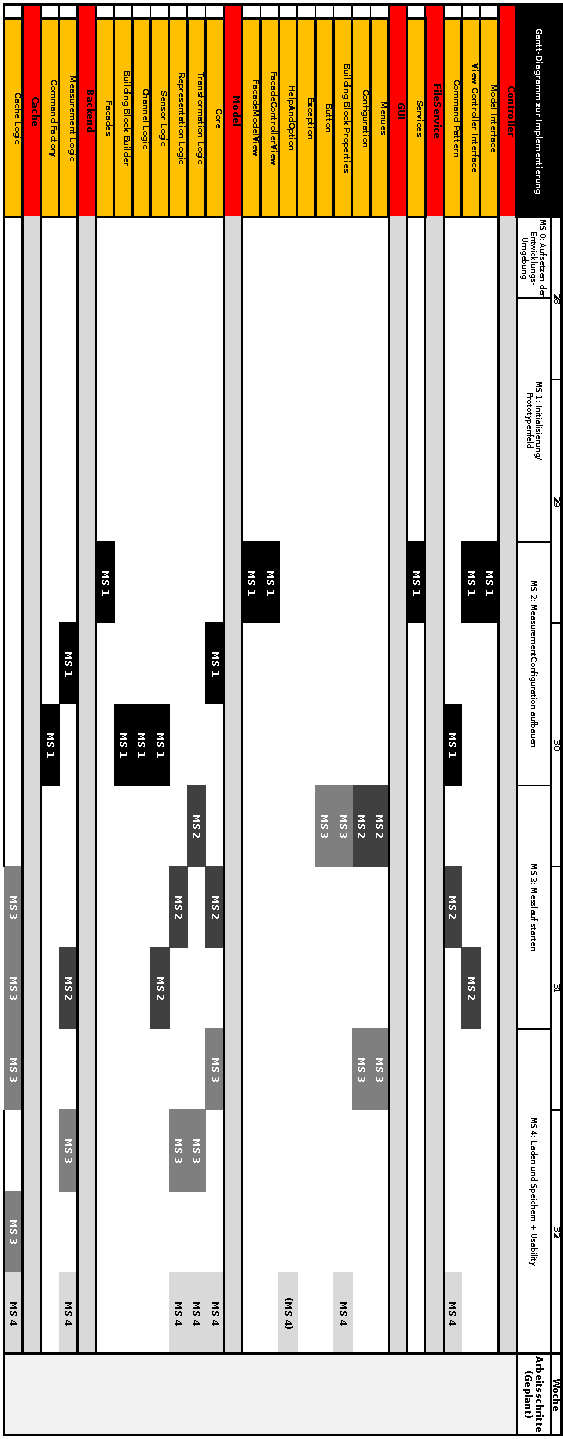
\includegraphics[height = 24cm]{Grafiken/Realer_Ablauf_der_Implementierung.pdf}
        \caption{Der reale Verlauf der Implementierung anhand eines Gantt-Diagramms}
        \label{reale}
    \end{center}
\end{figure}

\clearpage
\section{Glossar}\label{glossar}

\renewcommand*{\glossarysection}[2][]{}	% prevents double glossary section heading
\printnoidxglossaries				% generate pdf twice when adding new entries

\end{document}\grid
